% =====================================================================
%  第五章  离散化进程映像管理
% =====================================================================
\chapter{离散化进程映像管理}

\section{用户进程地址空间布局}
在新的页表与位示图基础设施之上，本章讨论进程映像在生命周期各关键时刻的管理。
首先要明确的是用户进程的地址空间布局。

尽管物理页框已经离散化，但\textbf{对用户程序而言，虚地址空间仍是连续的}：每个
用户进程拥有从 0 起的 8MB 虚拟空间（\texttt{MemoryDescriptor::USER\_SPACE\_SIZE
= 0x800000}），其中依次为代码段（text）、数据段（data）、堆（heap，向上扩展）与
栈（stack，自 8MB 顶端向下扩展）。这一布局与原系统保持一致，使得用户程序无需感知
物理页框是否连续——这正是分页机制"用页表把离散物理页拼接成连续虚拟空间"的核心价值，
也符合课设"离散化存储"的目标。

用户空间的映射由本进程私有的 1\# 用户页表承担。由于 0\# 用户页表覆盖低 4MB、1\#
用户页表覆盖高 4MB，而本设计中用户图像通常落在 1\# 页表管理的范围，因此在代码中
频繁出现如下页表下标换算：

\begin{lstlisting}[caption={用户虚地址到 1\# 页表项下标的换算},label={lst:pte-idx}]
// 虚地址 cr2 对应的 1# 用户页表项下标
unsigned int physicalBase =
    md.m_UserPageTableArray->m_Entrys[(cr2 >> 12) - 1024].m_PageBaseAddress;
\end{lstlisting}

\begin{figure}[H]
  \centering
  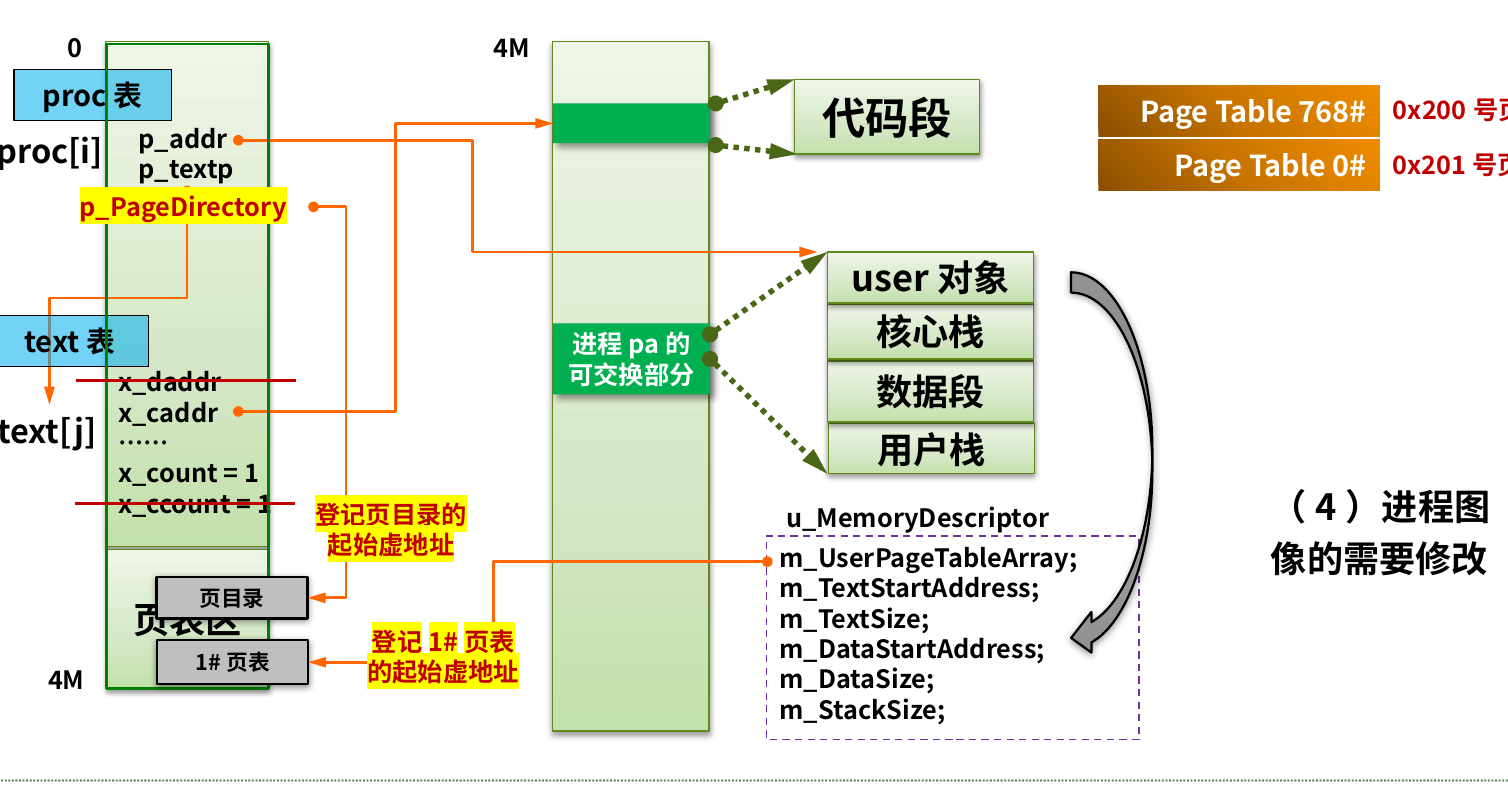
\includegraphics[width=0.9\textwidth]{figures/fig_proc_image.png}
  \caption{进程映像与页目录、页表、proc/text 表的关系（图源：课程设计 PPT slide 12）}
  \label{fig:proc-image}
\end{figure}

其中 \texttt{(cr2 >> 12)} 得到虚页号，减去 1024（即一张页表的表项数）是为了从 1\#
页表的角度换算下标——这一"减 1024"的约定贯穿了 fork、缺页、exec 等所有涉及用户页表
操作的路径。

\section{fork 与 COW 建立}
\texttt{fork} 是离散化改造中变化最大的路径之一。改造后的 \texttt{NewProc()} 不再
整体复制父进程图像，而是为子进程建立一套独立的页表结构，并与父进程\emph{共享}物理
页（写时复制）。其核心流程见代码清单~\ref{lst:newproc}。

\begin{lstlisting}[caption={fork (NewProc) 的 COW 建立},label={lst:newproc}]
// 对应源码 proc/ProcessManager.cpp :: NewProc
// NOTE 3: 为子进程建立私有页表与页目录
u.u_MemoryDescriptor.Initialize();                       // 分配子进程私有 1# 用户页表
PageTable *desPgTable = u.u_MemoryDescriptor.m_UserPageTableArray;
child->pPageDirectory   = ProcessManager::AllocPageDirectory(); // 子进程页目录
ProcessManager::InitProcPageDirectory(child, desPgTable);        // 填写页目录

// NOTE 4: 为子进程 PPDA 分配一页, 复制父进程 PPDA
unsigned long desAddress = userPageManager.AllocMemory(PageManager::PAGE_SIZE);
child->p_addr = desAddress;
Utility::CopySeg(current->p_addr, desAddress);

// NOTE 5 + COW: 复制父进程 1# 用户页表, 并把共享页置只读、引用计数加一
if (pgTable) {
    ProcessManager::ModifyPageTable(userPageManager, pgTable);   // 置 RW=0, Page[]++
    Utility::MemCopy((unsigned long)pgTable, (unsigned long)desPgTable, sizeof(PageTable));
}
\end{lstlisting}

其中 \texttt{ModifyPageTable()} 是 COW 建立的关键：它遍历父进程页表中所有"已存在且
可写"的表项，将其读写位 \texttt{m\_ReadWriter} 改为 0（只读），并对这些表项指向的
物理页框把引用计数 \texttt{Page[]} 加一：

\begin{lstlisting}[caption={ModifyPageTable: 共享页置只读并增加引用计数},label={lst:modify-pt}]
// 对应源码 proc/ProcessManager.cpp :: ModifyPageTable
void ProcessManager::ModifyPageTable(UserPageManager &userPageManager, PageTable* pgTable) {
    for (unsigned int j = 0; j < PageTable::ENTRY_CNT_PER_PAGETABLE; j++) {
        if (pgTable->m_Entrys[j].m_Present && pgTable->m_Entrys[j].m_ReadWriter) {
            pgTable->m_Entrys[j].m_ReadWriter = 0;                       // 置只读
            userPageManager.Page[pgTable->m_Entrys[j].m_PageBaseAddress]++; // 引用计数++
        }
    }
}
\end{lstlisting}

随后，父进程的整张 1\# 用户页表被原样复制给子进程（\texttt{MemCopy}）。于是 fork
完成后，父子两进程的页表完全相同，都把各自的数据/栈虚页指向\emph{同一批}物理页框，
且这些页框的页表项都被标记为只读、引用计数为 2。此时并没有发生任何用户图像的复制
（仅复制了页表这一页本身），这正是"写时复制"中"写时"之前的状态。

\section{page fault 中的 COW 处理}
COW 的真正复制发生在某一方尝试写入共享只读页时——这会触发缺页异常
（page fault），由 \texttt{Exception::PageFault()} 统一处理。该函数读取 \texttt{CR2}
得到缺页虚地址，判断这是否是一次"写只读共享页"的 COW 请求，并据此决定是直接放开
写权限还是复制新页，见代码清单~\ref{lst:cow-fault}。

\begin{lstlisting}[caption={page fault 中的 COW 处理},label={lst:cow-fault}]
// 对应源码 interrupt/Exception.cpp :: PageFault (节选)
unsigned char RW = md.m_UserPageTableArray->m_Entrys[(cr2 >> 12) - 1024].m_ReadWriter;
bool isRW = (cr2 >= md.m_DataStartAddress && cr2 < md.m_DataStartAddress + md.m_DataSize)
         || (cr2 >= USER_SPACE_SIZE - md.m_StackSize && cr2 < USER_SPACE_SIZE);
unsigned int physicalBase = md.m_UserPageTableArray->m_Entrys[(cr2 >> 12) - 1024].m_PageBaseAddress;

if (RW == 0 && userPageMgr.Page[physicalBase] >= 1 && isRW)   // 只读共享页 + 写数据/栈
{
    if (userPageMgr.Page[physicalBase] == 1) {                 // 仅本进程持有
        md.m_UserPageTableArray->m_Entrys[(cr2 >> 12) - 1024].m_ReadWriter = 1; // 直接放开写
        return;
    } else {                                                   // 还被其他进程共享
        --userPageMgr.Page[physicalBase];                      // 引用计数减一
        unsigned long newPage = userPageMgr.AllocMemory(M_PAGE_SIZE); // 分配新页
        md.m_UserPageTableArray->m_Entrys[(cr2 >> 12) - 1024].m_PageBaseAddress = newPage >> 12;
        md.m_UserPageTableArray->m_Entrys[(cr2 >> 12) - 1024].m_ReadWriter = 1; // 可写
        userPageMgr.Page[newPage >> 12] = 1;                   // 新页引用计数置 1
        Utility::CopySeg(physicalBase << 12, newPage);         // 复制原页内容
        return;
    }
}
\end{lstlisting}

这里体现了 COW 的两个分支。当 \texttt{Page[physicalBase] == 1} 时，说明该物理页虽然
被标记为只读共享，但实际上只剩当前进程一个引用者（其他进程已先后触发 COW 分离），
此时无需复制，直接把页表项的读写位置 1 即可；当 \texttt{Page[physicalBase] > 1} 时，
该页仍被其他进程共享，当前进程必须分配一个新物理页、复制原页内容、把页表项重定向到
新页，并把原页的引用计数减一。\texttt{isRW} 的判断确保只有对数据段或栈段的写入才走
COW 路径——代码段（text）本身就该只读共享，其写入应被视为非法访问。

若缺页既非 COW 请求、也非合法的栈扩展，则按非法内存访问处理：用户态越界发送
\texttt{SIGSEGV} 信号，内核态则 \texttt{Panic}。

\section{exec 图像改换与参数栈构造}
\texttt{exec} 是另一条高度改造的路径。原系统 \texttt{exec} 需要把新程序图像搬运到
一段连续的用户内存；改造后，本设计为\emph{新用户栈}分配物理页框，在其上接纳命令行
参数，然后直接建立用户页表映射，\emph{省去了整段图像的内存复制}。

\texttt{Exec()} 的参数栈构造是其精巧之处。由于用户程序尚未运行、其私有页表还未建立，
代码\emph{借用}全局共享的 0\# 用户页表作为临时窗口：先为新栈分配连续物理页框
（\texttt{trueStack}），把它们临时挂到 0\# 页表的前几项，使内核能通过低地址访问到
这些栈页；随后自顶向下在栈上依次写入命令行字符串、\texttt{argv[]} 指针数组、结束标志
与 \texttt{argc}；最后撤销对 0\# 页表的临时借用，恢复其原貌。关键代码见清单~%
\ref{lst:exec-stack}。

\begin{lstlisting}[caption={exec 借用 0\# 页表构造参数栈},label={lst:exec-stack}]
// 对应源码 proc/ProcessManager.cpp :: Exec (节选)
int pages = (parser.StackSize + PAGE_SIZE - 1) >> 12;
unsigned long trueStack = (userPgMgr.AllocMemory(pages << 12)) >> 12; // 为新栈分配物理页框
PageTableEntry *tempEntrys = (PageTableEntry *)Machine::Instance().GetUserPageTableArray();
for (int i = 1; i <= pages; i++, trueStack++) {           // 临时挂到 0# 页表
    tempEntrys[i].m_Present = 1; tempEntrys[i].m_ReadWriter = true;
    tempEntrys[i].m_PageBaseAddress = trueStack;
}
u.u_MemoryDescriptor.MapToPageTable();                    // 刷新使映射生效
// ... 自顶向下写入 argv 字符串、argv[] 指针数组、argc ...
for (int i = 1; i <= pages; i++) {                        // 恢复 0# 页表, 撤销借用
    tempEntrys[i].m_Present = 0; tempEntrys[i].m_ReadWriter = false;
}
u.u_MemoryDescriptor.MapToPageTable();
\end{lstlisting}

参数栈构造完成后，\texttt{Exec} 释放旧的正文段（\texttt{XFree}）、数据段与栈段，
再按 PE 文件头给出的新 \texttt{text}/\texttt{data}/\texttt{stack} 尺寸，分别为数据段、
栈段分配物理页框并填写私有 1\# 用户页表项；正文段则走共享路径（见下文）。最终通过
\texttt{Relocate} 完成重定位，并把返回地址设为程序入口，使系统调用返回 ring3 后从
新程序开始执行。整个过程中，用户图像不需要被整体搬运，仅需写入命令行参数与建立
页表映射。

\section{exit 与共享 text 释放}
进程退出时，需要释放其占用的物理页框。数据段与栈段页框由引用计数
（\texttt{Page[]--}）配合 \texttt{FreeMemory} 释放；而正文段由于可能被多个进程共享，
其释放由 \texttt{Text} 结构中的两个计数器控制（\texttt{proc/Text.cpp}）：

\begin{itemize}
  \item \texttt{x\_ccount}：当前在内存中（已加载）引用该正文段的进程数；
  \item \texttt{x\_count}：总体（含潜在换出）引用该正文段的进程数。
\end{itemize}

\texttt{Text::XccDec()} 在每次退出时被调用，先递减 \texttt{x\_ccount}，只有当它降到
0（即内存中已无进程使用该正文段）时，才真正释放正文段各页的物理页框；\texttt{XFree()}
则在 \texttt{XccDec} 基础上进一步判断 \texttt{x\_count}，当它也降为 0 时释放对应的
swap 副本与 inode。这种双层计数保证了正文段的物理页只在\emph{所有}共享者都退出后才
被回收，避免误释放仍被他进程使用的代码页。

\section{wait 写 status 时的 COW 处理}
父进程通过 \texttt{wait} 回收子进程时，往往需要把子进程的退出状态写入子进程的用户
地址空间。若该目标页恰好是 fork 时建立的 COW 共享只读页，这一写入会自然地触发缺页
异常，进而走与第 5.3 节完全相同的 COW 处理路径：分配新页、复制内容、重定向页表项。

也就是说，COW 机制并不专属于某一条系统调用，而是由 \texttt{PageFault} 统一兜底——
任何对只读共享页的写入，无论来自 fork 后的父子、wait 的状态写回，还是其他路径，都会
被同一套引用计数判断与复制逻辑接管。这种"机制统一、调用无关"的设计，使得 COW 能够
一致地覆盖进程生命周期中所有涉及共享页写入的场景。需要指出的是，COW 判断的地址范围
（\texttt{isRW}）必须准确覆盖数据段与栈段，否则会出现共享页无法及时分离的问题，
这一点将在第七章 7.2 节作为一个实际调试案例讨论。

\section{堆扩展与栈扩展}
离散化模型下，堆与栈的动态扩展变得十分自然。\texttt{SBreak}（响应 \texttt{brk}
系统调用）扩展堆时，只需为新虚页分配空闲物理页框并在私有页表中建立映射，无需像
连续模型那样保证与既有区域物理相邻；\texttt{SStack} 处理栈的自动向下扩展——当访问
超越当前栈顶但仍在合理范围内的地址时，\texttt{PageFault} 会判定为合法的栈扩展
（见第 5.3 节末尾的栈扩展分支），调用 \texttt{SStack} 补齐缺失的栈页。

由于每次扩展都只涉及"分配新页框 + 更新私有页表项"两步，不依赖连续物理内存，离散化
模型从根本上消除了原连续模型下扩展可能因找不到连续区而失败的问题，也为按需分配
（demand paging）提供了天然支持。

\subsection*{运行验证}
执行 \texttt{/bin/echo hello}，程序正确输出参数 \texttt{hello}（图~\ref{fig:run-echo}），
验证了 \texttt{exec} 借用 0\# 页表构造参数栈、向新程序传递 \texttt{argc}/\texttt{argv}
的机制。执行 \texttt{/bin/forks}，程序连续 \texttt{fork} 创建多个子进程（PID 依次
递增），父进程经 \texttt{wait} 逐个回收（图~\ref{fig:run-forks}），验证了 fork 写时
复制建立共享页、进程映像离散存放与按引用回收在多次进程创建下的正确性。

\begin{figure}[H]
  \centering
  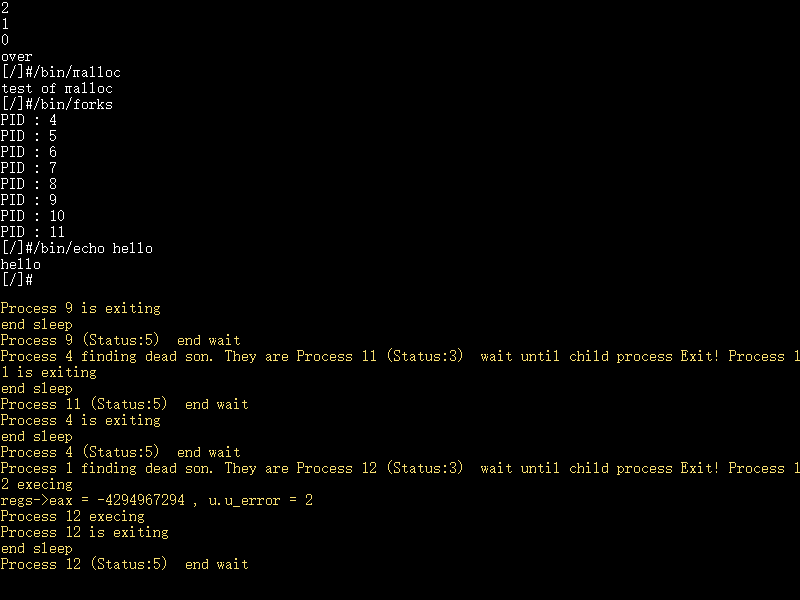
\includegraphics[width=0.85\textwidth]{figures/run_echo.png}
  \caption{运行 /bin/echo hello：exec 命令行参数传递验证}
  \label{fig:run-echo}
\end{figure}

\begin{figure}[H]
  \centering
  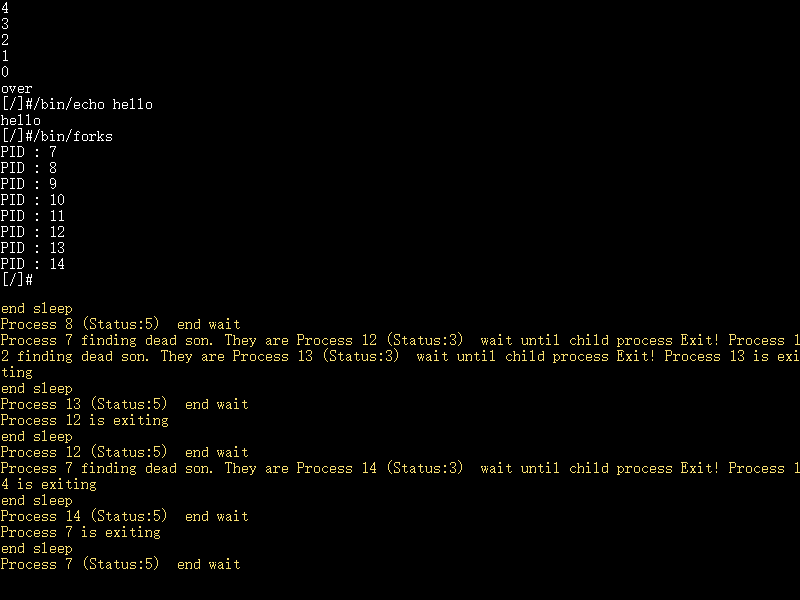
\includegraphics[width=0.85\textwidth]{figures/run_forks.png}
  \caption{运行 /bin/forks：多进程创建与进程映像离散化验证}
  \label{fig:run-forks}
\end{figure}

\section{本章小结}
本章把进程映像管理全面转向离散模型：fork 用 COW 延迟复制，仅在真正写入时经
\texttt{PageFault} 分离共享页；exec 用借用 0\# 页表构造参数栈、直接挂用户页表，省去
图像搬运；text 段用 \texttt{x\_ccount}/\texttt{x\_count} 双计数实现共享与按引用释放；
堆栈扩展则降级为"分配页框 + 更新页表"。配合第四章的位示图与引用计数，物理页的生命
周期得以由共享语义而非单个页表项正确管理，"离散存放 + 按需分配"的进程映像管理目标
至此基本达成。
